\definecolor{amministratore}{RGB}{51,102,204}
\definecolor{analista}{RGB}{255,153,0}
\definecolor{progettista}{RGB}{153,0,153}
\definecolor{programmatore}{RGB}{7,55,99}
\definecolor{responsabile}{RGB}{220,57,18}
\definecolor{verificatore}{RGB}{16,150,24}

\definecolor{Pianificate}{RGB}{51,102,204}
\definecolor{Consumate}{RGB}{32,18,77}

\pgfplotsset{
ybar, 
stack plots=false,
enlargelimits =0.10,
legend style ={at={(0.5,-0.5)},
anchor=north,
legend columns=-1},
ylabel={Ore},
xtick=data,
x tick label style={rotate=45,anchor=east},
symbolic x coords={Amministratore, Analista, Progettista, Programmatore, Responsabile, Verificatore},
}

\section{Prospetto economico}

In questa sezione è presentato il prospetto economico del progetto \ProjectName{}, suddiviso per periodi. Per ogni periodo sono indicate le ore preventivate per ogni ruolo impiegato.
Il costo è calcolato utilizzando i dati della tabella al paragrafo \ref{tabellacostiruolo}.

\subsection{Analisi}

A scopo di trasparenza viene redatto il prospetto economico riguardante il periodo di Analisi dei requisiti, ma si precisa che le ore spese in questo periodo sono a carico del fornitore e non del proponente.

\begin{table}[H]
	\centering
	\begin{tabular}{ l c c }
	\textbf{Ruolo} & \textbf{Ore} & \textbf{Costo} \\
	\hline
		Amministratore & 30 & 600 € \\
	Analista & 58 & 1450 € \\
	Progettista & 9 & 198 € \\
	Programmatore & 0 & 0 € \\
	Responsabile & 14 & 420 € \\
	Verificatore & 31 & 465 € \\
\hline
	Totale & 142 & 3133 € \\
\hline

	\end{tabular}
	\caption{Ore e costo per ruolo, periodo di Analisi}
	\end{table}

I seguenti grafici mostrano il peso orario e di costo di ogni ruolo in questo periodo.

\begin{figure}[H]
\begin{tikzpicture}

	\pie[text=legend, color={amministratore, analista, progettista, programmatore, responsabile, verificatore}]{21.1/Amministratore, 40.8/Analista, 6.3/Progettista, ./Programmatore, 9.9/Responsabile, 21.8/Verificatore}


\end{tikzpicture}
\caption{Ore per ruolo, periodo di Analisi}
\end{figure}

\begin{figure}[H]
\begin{tikzpicture}

	\pie[text=legend, color={amministratore, analista, progettista, programmatore, responsabile, verificatore}]{19.2/Amministratore, 46.3/Analista, 6.3/Progettista, ./Programmatore, 13.4/Responsabile, 14.8/Verificatore}


\end{tikzpicture}
\caption{Costo per ruolo, periodo di Analisi}
\end{figure}

Di seguito viene invece presentato il consuntivo relativo al periodo di \textit{Analisi}. La tabella sottostante riporta le ore preventivate e le ore effettivamente impiegate (riportate tra parentesi) per ciascun ruolo.

\begin{table}[H]
\centering
\begin{tabular}{lccccccc}
\toprule
    \textbf{Ruolo}  & \textbf{Ore} & \textbf{Costo} \\
    \midrule
    
    		Amministratore & 30 (+0) & 600 (+0) € \\
	Analista & 58 (-8) & 1450 (-200) € \\
	Progettista & 9 (-1) & 198 (-22) € \\
	Programmatore & 0 (+0) & 0 (+0) € \\
	Responsabile & 14 (+1) & 420 (+30) € \\
	Verificatore & 31 (+9) & 465 (+135) € \\
\hline
\textbf{Totale consuntivo} & +141 & +3190 € \\
\textbf{Totale preventivo} & +142 & +3133 € \\
\textbf{Differenza dei totali} & +1 & -57 € \\

    
    \bottomrule
\end{tabular}
\caption{Differenza preventivo consuntivo per ruolo, periodo di Analisi}
\end{table}

Viene di seguito incluso il grafico che illustra la differenza tra ore preventivate e ore effettivamente impiegate per ciascun ruolo nel periodo di \textit{Analisi}.

\begin{figure}[H]
\centering
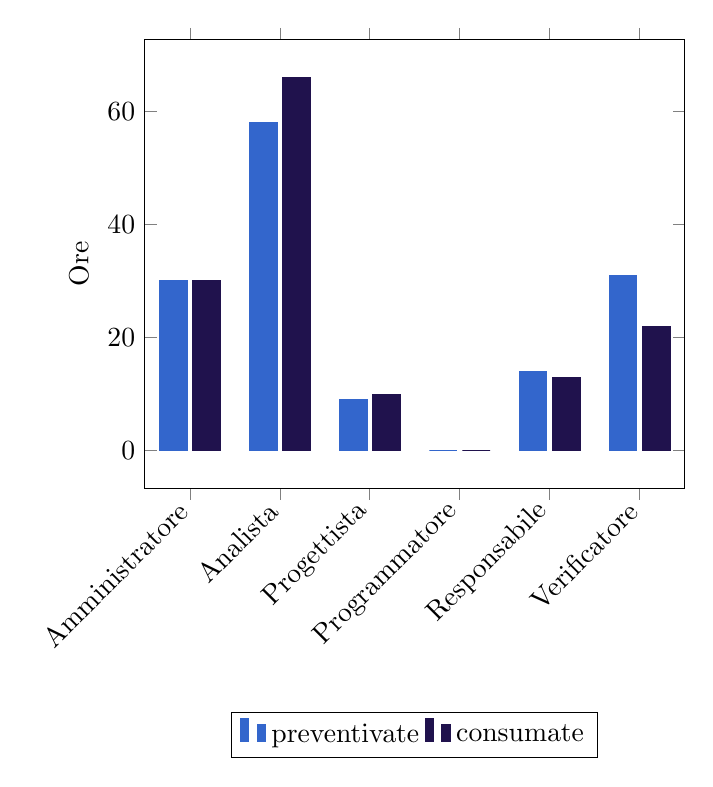
\begin{tikzpicture}
\begin{axis}
\addplot+[color=Pianificate] plotcoordinates {(Amministratore,30)(Analista,58)(Progettista,9)(Programmatore,0)(Responsabile,14)(Verificatore,31)};
\addplot+[color=Consumate] plotcoordinates {(Amministratore,30)(Analista,66)(Progettista,10)(Programmatore,0)(Responsabile,13)(Verificatore,22)};

\legend{preventivate,consumate}
\end{axis}
\end{tikzpicture}
\caption{Differenza preventivo consuntivo per ruolo, periodo di analisi}
\end{figure}

\subsection{Progettazione architetturale}

Nel periodo di Progettazione architetturale le ore per ogni ruolo sono state cosi suddivise:

\begin{table}[H]
	\centering
	\begin{tabular}{ l c c }
	\textbf{Ruolo} & \textbf{Ore} & \textbf{Costo} \\
	\hline
	
			Amministratore & 58 & 1160 € \\
	Analista & 22 & 550 € \\
	Progettista & 112 & 2464 € \\
	Programmatore & 0 & 0 € \\
	Responsabile & 27 & 810 € \\
	Verificatore & 74 & 1110 € \\
\hline
	Totale & 293 & 6094 € \\
\hline

	
	\end{tabular}
	\caption{Ore e costo per ruolo, periodo di Progettazione architetturale}
	\end{table}
	
I seguenti grafici mostrano il peso orario e di costo di ogni ruolo in questo periodo.

\begin{figure}[H]
\begin{tikzpicture}

	\pie[sum=auto, text=legend]{48/Amministratore, 24/Analista, 70/Progettista, 19.0/Responsabile, 42/Verificatore}


\end{tikzpicture}
\caption{Ore per ruolo, periodo di Progettazione architetturale}
\end{figure}

\begin{figure}[H]
\begin{tikzpicture}

	\pie[text=legend, color={amministratore, analista, progettista, programmatore, responsabile, verificatore}]{32.9/Amministratore, 9.2/Analista, 39.6/Progettista, ./Programmatore, 8.7/Responsabile, 9.6/Verificatore}


\end{tikzpicture}
\caption{Costo per ruolo, periodo di Progettazione architetturale}
\end{figure}

La tabella sottostante riporta le ore preventivate e le ore effettivamente impiegate (riportate tra parentesi) per ciascun ruolo presente nel periodo di \textit{Progettazione architetturale}.

\begin{table}[H]
\centering
\begin{tabular}{lccccccc}
\toprule
    \textbf{Ruolo}  & \textbf{Ore} & \textbf{Costo} \\
    \midrule
    
    		Amministratore & 42 (+0) & 840 (+0) € \\
	Analista & 24 (+0) & 600 (+0) € \\
	Progettista & 108 (+0) & 2376 (+0) € \\
	Programmatore & 0 (+0) & 0 (+0) € \\
	Responsabile & 26 (-3) & 780 (-90) € \\
	Verificatore & 78 (+0) & 1170 (+0) € \\
\hline
\textbf{Totale consuntivo} & +281 & +5856 € \\
\textbf{Totale preventivo} & +278 & +5766 € \\
\textbf{Differenza dei totali} & -3 & -90 € \\

    
    \bottomrule
\end{tabular}
\caption{Differenza preventivo consuntivo per ruolo, periodo di Progettazione Architetturale}
\end{table}

Viene di seguito incluso il grafico che illustra la differenza tra ore preventivate e ore effettivamente impiegate per ciascun ruolo nel periodo di \textit{Progettazione architetturale}.

\begin{figure}[H]
\centering
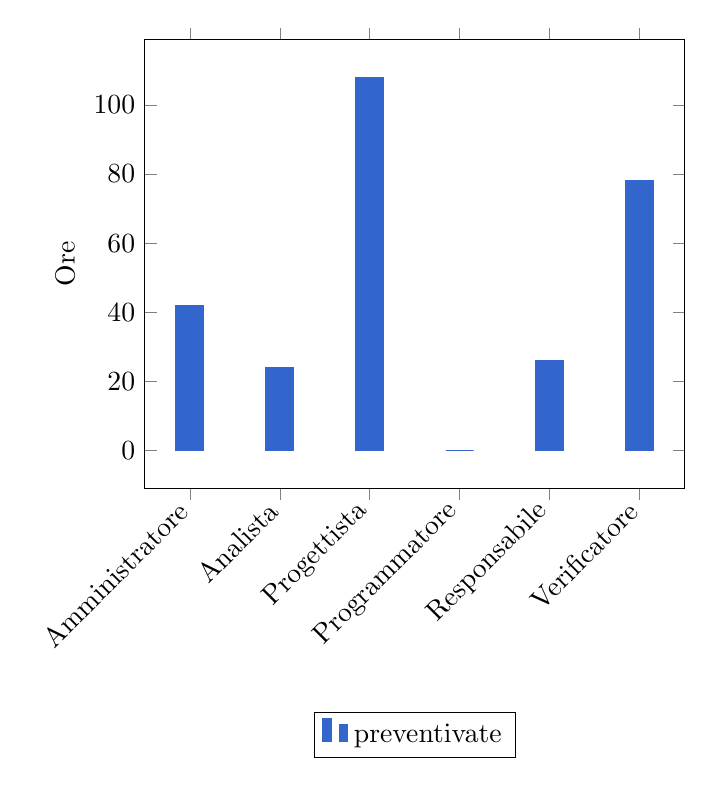
\begin{tikzpicture}
\begin{axis}
\addplot+[color=Pianificate] coordinates {(Amministratore,42)(Analista,24)(Progettista,108)(Programmatore,0)(Responsabile,26)(Verificatore,78)};

\legend{preventivate,consumate}
\end{axis}
\end{tikzpicture}
\caption{Differenza preventivo consuntivo per ruolo, periodo di progettazione architetturale}
\end{figure}

\subsection{Progettazione di dettaglio e codifica}

Nel periodo di Progettazione di dettaglio e codifica le ore per ogni ruolo sono state cosi suddivise:

\begin{table}[H]
	\centering
	\begin{tabular}{ l c c }
	\textbf{Ruolo} & \textbf{Ore} & \textbf{Costo} \\
	\hline
	
			Amministratore & 42 & 840 € \\
	Analista & 8 & 200 € \\
	Progettista & 66 & 1452 € \\
	Programmatore & 126 & 1890 € \\
	Responsabile & 4 & 120 € \\
	Verificatore & 54 & 810 € \\
\hline
	Totale & 300 & 5312 € \\
\hline

	
	\end{tabular}
	\caption{Ore e costo per ruolo, periodo di Progettazione di dettaglio e codifica}
	\end{table}

I seguenti grafici mostrano il peso orario e di costo di ogni ruolo in questo periodo.

\begin{figure}[H]
\begin{tikzpicture}

	\pie[sum=auto, text=legend]{38/Amministratore, 8/Analista, 120/Progettista, 132/Programmatore, ./Responsabile, 90/Verificatore}


\end{tikzpicture}
\caption{Ore per ruolo, periodo di Progettazione di dettaglio e codifica}
\end{figure}

\begin{figure}[H]
\begin{tikzpicture}

	\pie[text=legend, color={amministratore, analista, progettista, programmatore, responsabile, verificatore}]{16.4/Amministratore, 3.8/Analista, 27.6/Progettista, 36.0/Programmatore, 2.3/Responsabile, 14.0/Verificatore}


\end{tikzpicture}
\caption{Costo per ruolo, periodo di Progettazione di dettaglio e codifica}
\end{figure}

La tabella sottostante riporta le ore preventivate e le ore effettivamente impiegate (riportate tra parentesi) per ciascun ruolo presente nel periodo di \textit{Progettazione di dettaglio e codifica}.

\begin{table}[H]
\centering
\begin{tabular}{lccccccc}
\toprule
    \textbf{Ruolo}  & \textbf{Ore} & \textbf{Costo} \\
    \midrule
    
    		Amministratore & 42 (+0) & 840 (+0) € \\
	Analista & 8 (+0) & 200 (+0) € \\
	Progettista & 66 (+0) & 1452 (+0) € \\
	Programmatore & 126 (+0) & 1890 (+0) € \\
	Responsabile & 4 (+0) & 120 (+0) € \\
	Verificatore & 46 (-4) & 690 (-60) € \\
\hline
\textbf{Totale consuntivo} & +296 & +5252 € \\
\textbf{Totale preventivo} & +292 & +5192 € \\
\textbf{Differenza dei totali} & -4 & -60 € \\

    
    \bottomrule
\end{tabular}
\caption{Differenza preventivo consuntivo per ruolo, periodo di Progettazione di dettaglio e codifica}
\end{table}

Viene di seguito incluso il grafico che illustra la differenza tra ore preventivate e ore effettivamente impiegate per ciascun ruolo nel periodo di \textit{Progettazione di dettaglio e codifica}.

\begin{figure}[H]
\centering
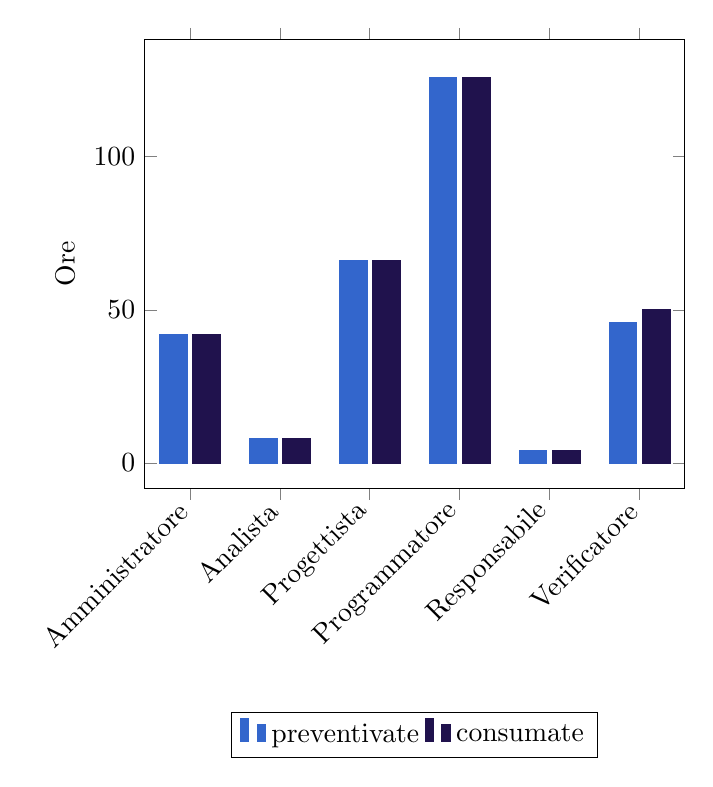
\begin{tikzpicture}
\begin{axis}
\addplot+[color=Pianificate] plotcoordinates {(Amministratore,42.0)(Analista,8)(Progettista,66)(Programmatore,126)(Responsabile,4)(Verificatore,46.0)};
\addplot+[color=Consumate] plotcoordinates {(Amministratore,42.0)(Analista,8)(Progettista,66)(Programmatore,126.0)(Responsabile,4)(Verificatore,50.0)};

\legend{preventivate,consumate}
\end{axis}
\end{tikzpicture}
\caption{Differenza preventivo consuntivo per ruolo, periodo di progettazione di dettaglio e codifica}
\end{figure}

\subsection{Validazione}

Nel periodo di Validazione le ore per ogni ruolo sono state cosi suddivise:

\begin{table}[H]
	\centering
	\begin{tabular}{ l c c }
	\textbf{Ruolo} & \textbf{Ore} & \textbf{Costo} \\
	
			Amministratore & 16 & 320 € \\
	Analista & 0 & 0 € \\
	Progettista & 8 & 176 € \\
	Programmatore & 0 & 0 € \\
	Responsabile & 8 & 240 € \\
	Verificatore & 98 & 1470 € \\
\hline
	Totale & 130 & 2206 € \\
\hline

	
	\end{tabular}
	\caption{Ore e costo per ruolo, periodo di Validazione}
	\end{table}

I seguenti grafici mostrano il peso orario e di costo di ogni ruolo in questa periodo.

\begin{figure}[H]
\begin{tikzpicture}

	\pie[sum=auto, text=legend]{30/Amministratore, ./Analista, ./Progettista, ./Programmatore, ./Responsabile, 110/Verificatore}


\end{tikzpicture}\caption{Ore per ruolo, periodo di Validazione}
\end{figure}

\begin{figure}[H]
\begin{tikzpicture}

	\pie[text=legend, color={amministratore, analista, progettista, programmatore, responsabile, verificatore}]{14.5/Amministratore, ./Analista, 8.0/Progettista, ./Programmatore, 10.9/Responsabile, 66.6/Verificatore}


\end{tikzpicture}
\caption{Costo per ruolo, periodo di Validazione}
\end{figure}

La tabella sottostante riporta le ore preventivate e le ore effettivamente impiegate (riportate tra parentesi) per ciascun ruolo presente nel periodo di \textit{Validazione}.

\begin{table}[H]
\centering
\begin{tabular}{lccccccc}
\toprule
    \textbf{Ruolo}  & \textbf{Ore} & \textbf{Costo} \\
    \midrule
    
    		Amministratore & 10 (+0) & 200 (+0) € \\
	Analista & 0 (+0) & 0 (+0) € \\
	Progettista & 16 (+0) & 352 (+0) € \\
	Programmatore & 18 (+0) & 270 (+0) € \\
	Responsabile & 4 (+0) & 120 (+0) € \\
	Verificatore & 89 (+0) & 1335 (+0) € \\
\hline
\textbf{Totale consuntivo} & +137 & +2277 € \\
\textbf{Totale preventivo} & +137 & +2277 € \\
\textbf{Differenza dei totali} & +0 & +0 € \\

    
    \bottomrule
\end{tabular}
\caption{Differenza preventivo consuntivo per ruolo, periodo di Validazione}
\end{table}

Viene di seguito incluso il grafico che illustra la differenza tra ore preventivate e ore effettivamente impiegate per ciascun ruolo nel periodo di \textit{Validazione}.

\begin{figure}[H]
\centering
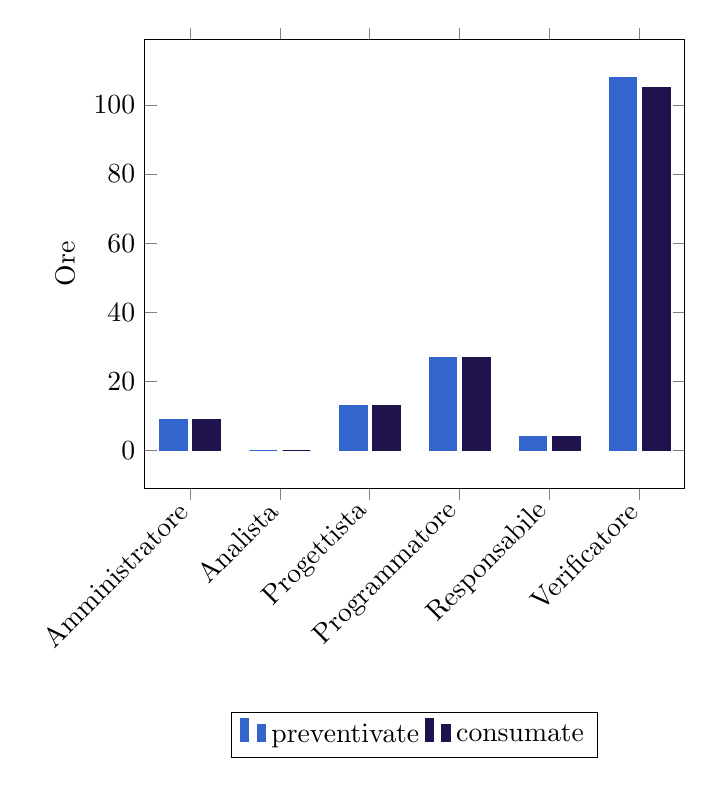
\begin{tikzpicture}
\begin{axis}
\addplot+[color=Pianificate] plotcoordinates {(Amministratore,9.0)(Analista,0)(Progettista,13.0)(Programmatore,27.0)(Responsabile,4)(Verificatore,108.0)};
\addplot+[color=Consumate] plotcoordinates {(Amministratore,9.0)(Analista,0)(Progettista,13.0)(Programmatore,27.0)(Responsabile,4)(Verificatore,105.066666667)};

\legend{preventivate,consumate}
\end{axis}
\end{tikzpicture}
\caption{Differenza preventivo consuntivo per ruolo, periodo di Validazione}
\end{figure}

\subsection{Totale}

In totale le ore per ogni ruolo sono state cosi suddivise:

\begin{table}[H]
	\centering
	\begin{tabular}{ l c c }
	\textbf{Ruolo} & \textbf{Ore} & \textbf{Costo} \\
	\hline
	
			Amministratore & 102 & 2040 € \\
	Analista & 30 & 750 € \\
	Progettista & 184 & 4048 € \\
	Programmatore & 126 & 1890 € \\
	Responsabile & 35 & 1050 € \\
	Verificatore & 224 & 3360 € \\
\hline
	Totale & 701 & 13138 € \\
\hline

	
	\end{tabular}
	\caption{Ore e costo per ruolo, riassunto progetto}
	\end{table}

Il seguente grafico mostra il costo di ogni ruolo durante tutto lo svolgimento del progetto, escluso il periodo di Analisi dei requisiti.

\begin{figure}[H]
\begin{tikzpicture}

	\pie[text=legend, color={amministratore, analista, progettista, programmatore, responsabile, verificatore}]{13.9/Amministratore, 6.0/Analista, 31.5/Progettista, 14.2/Programmatore, 7.7/Responsabile, 26.7/Verificatore}


\end{tikzpicture}
\caption{Costo per ruolo}
\end{figure}

La tabella sottostante riporta le ore preventivate e le ore effettivamente impiegate (riportate tra parentesi) per ciascun ruolo presente nel periodo totale corrente alla consegna del presente documento, escluso il periodo di Analisi dei requisiti.

\begin{table}[H]
\centering
\begin{tabular}{lccccccc}
\toprule
    \textbf{Ruolo}  & \textbf{Ore} & \textbf{Costo} \\
    \midrule
    
    		Amministratore & 83 (+4) & 1660 (+77) € \\
	Analista & 32 (+2) & 800 (+54) € \\
	Progettista & 174 (-12) & 3828 (-268) € \\
	Programmatore & 126 (+0) & 1890 (+0) € \\
	Responsabile & 30 (+3) & 900 (+90) € \\
	Verificatore & 132 (+8) & 1980 (+124) € \\
\hline
\textbf{Totale consuntivo} & +572 & +10981 € \\
\textbf{Totale preventivo} & +577 & +11058 € \\
\textbf{Differenza dei totali} & +5 & +77 € \\

    
    \bottomrule
\end{tabular}
\caption{Differenza preventivo consuntivo per ruolo, totale corrente}
\end{table}

\begin{figure}[H]
\centering
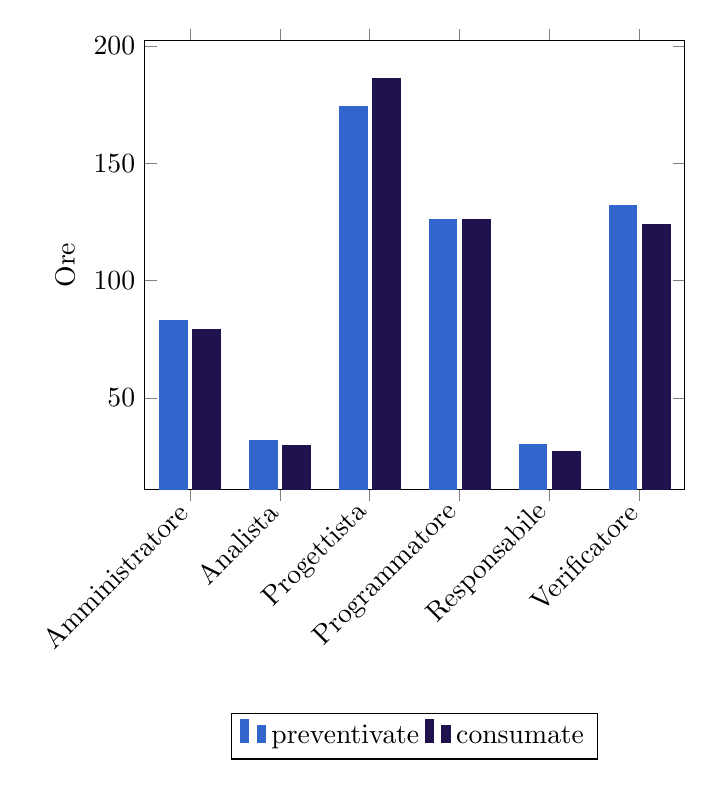
\begin{tikzpicture}
\begin{axis}
\addplot+[color=Pianificate] plotcoordinates {(Amministratore,83.0)(Analista,32)(Progettista,174)(Programmatore,126)(Responsabile,30)(Verificatore,132)};
\addplot+[color=Consumate] plotcoordinates {(Amministratore,79.1666666667)(Analista,29.8333333333)(Progettista,186.166666667)(Programmatore,126)(Responsabile,27.0)(Verificatore,123.75)};

\legend{preventivate,consumate}
\end{axis}
\end{tikzpicture}
\caption{Differenza preventivo consuntivo per ruolo, totale corrente}
\end{figure}